\begin{figure}
	\subfloat[Model 1 is in group A (rank=2, bad match).]
	{
		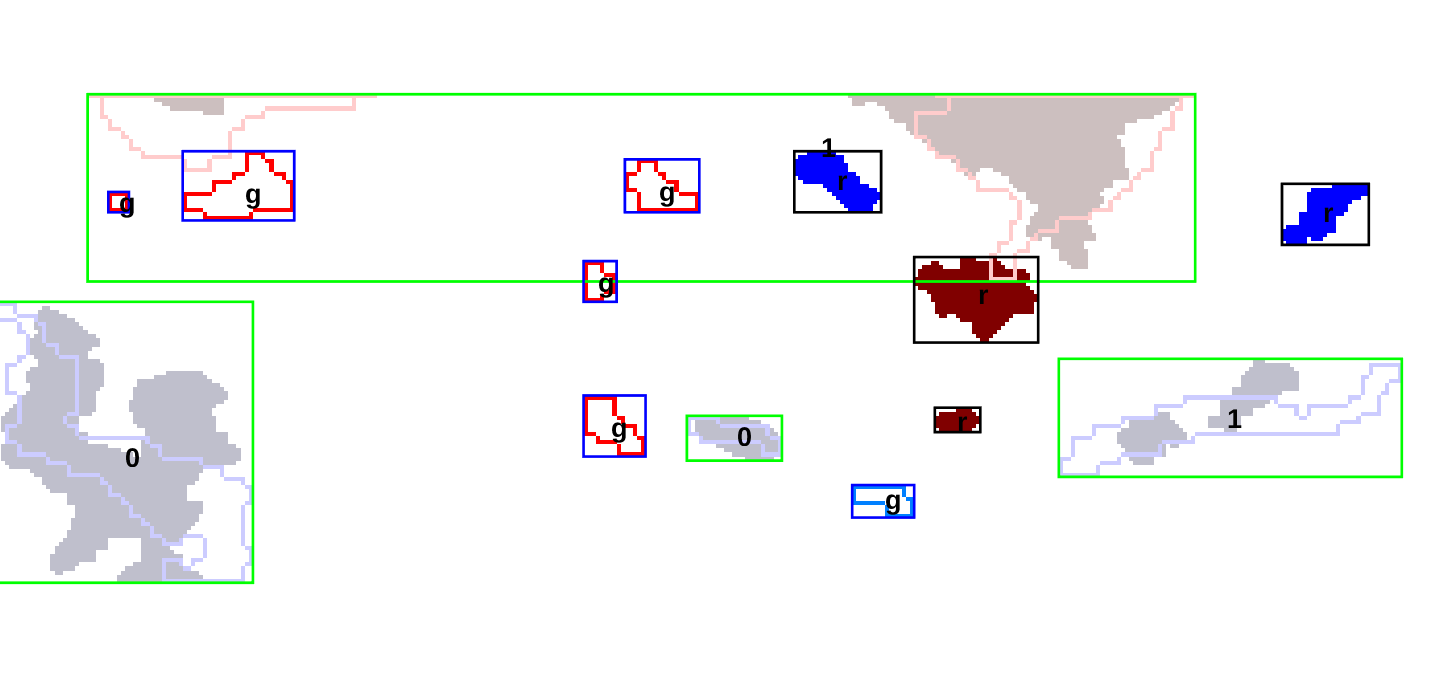
\includegraphics[width=0.45\linewidth]{pictures/thesis/chapter3/classificationProtocol/20110120model1Matched_cropped.png}
		\label{subfig:m1g1}
	}
	~\subfloat[Model 6 is in group A (rank=2, bad match).]
	{
		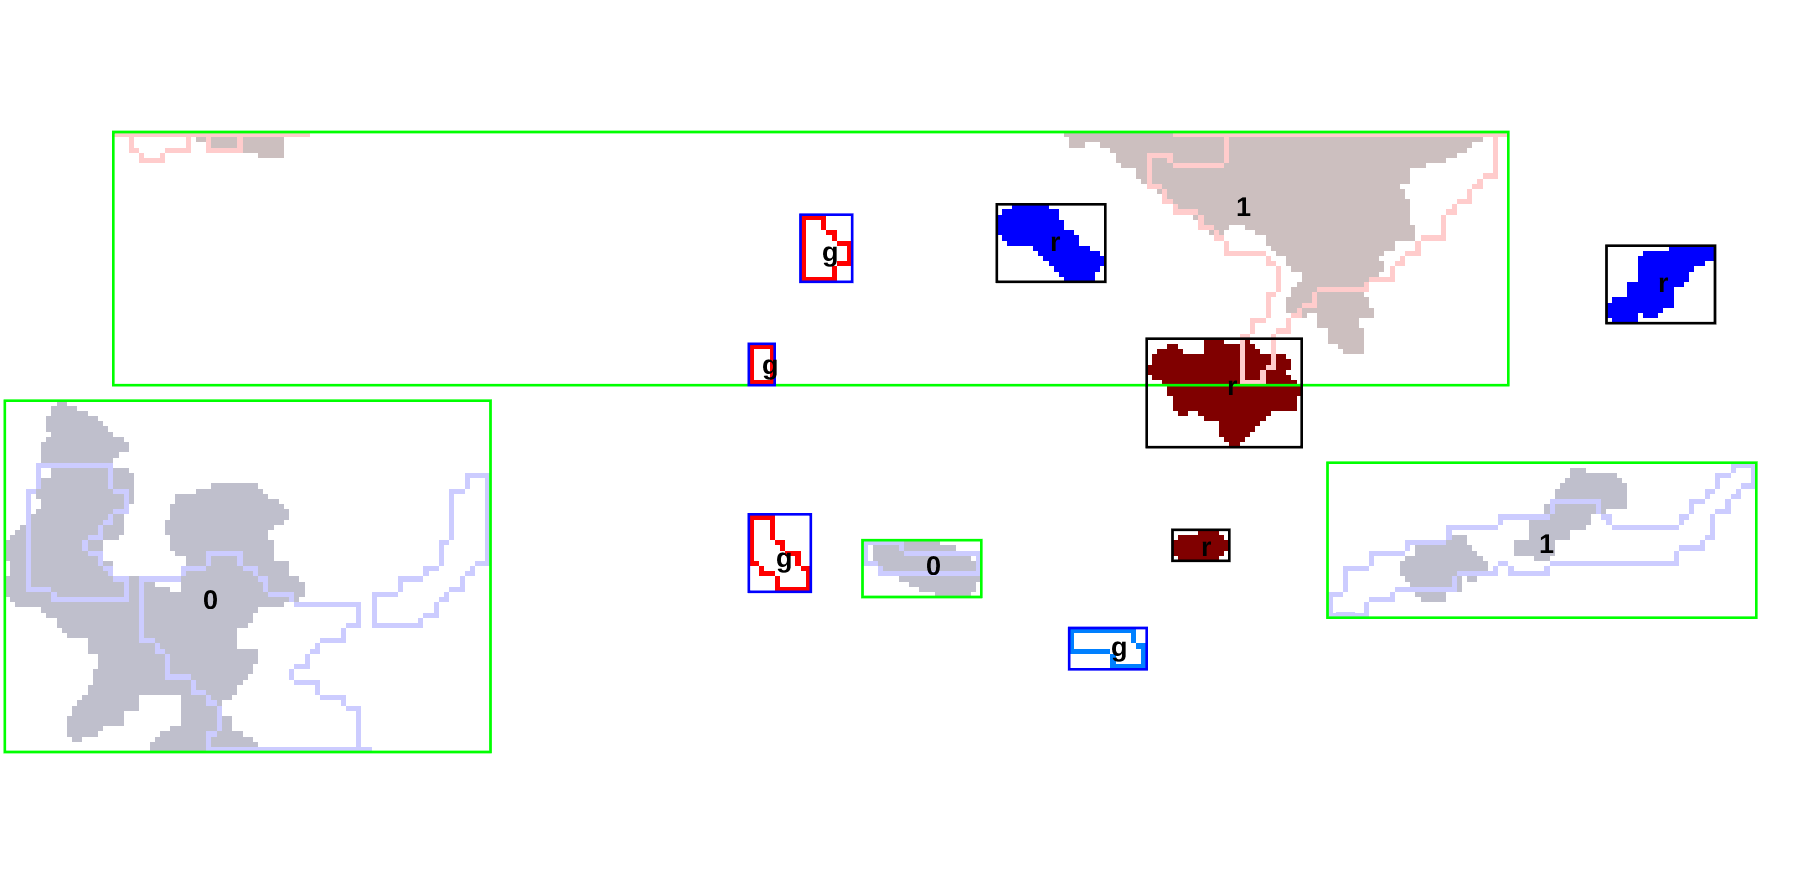
\includegraphics[width=0.45\linewidth]{pictures/thesis/chapter3/classificationProtocol/20110120model6Matched_cropped.png}
		\label{subfig:m6g1}
		
	}
	
	\subfloat[Model 8 is in group A (rank=2, bad match).]
	{
		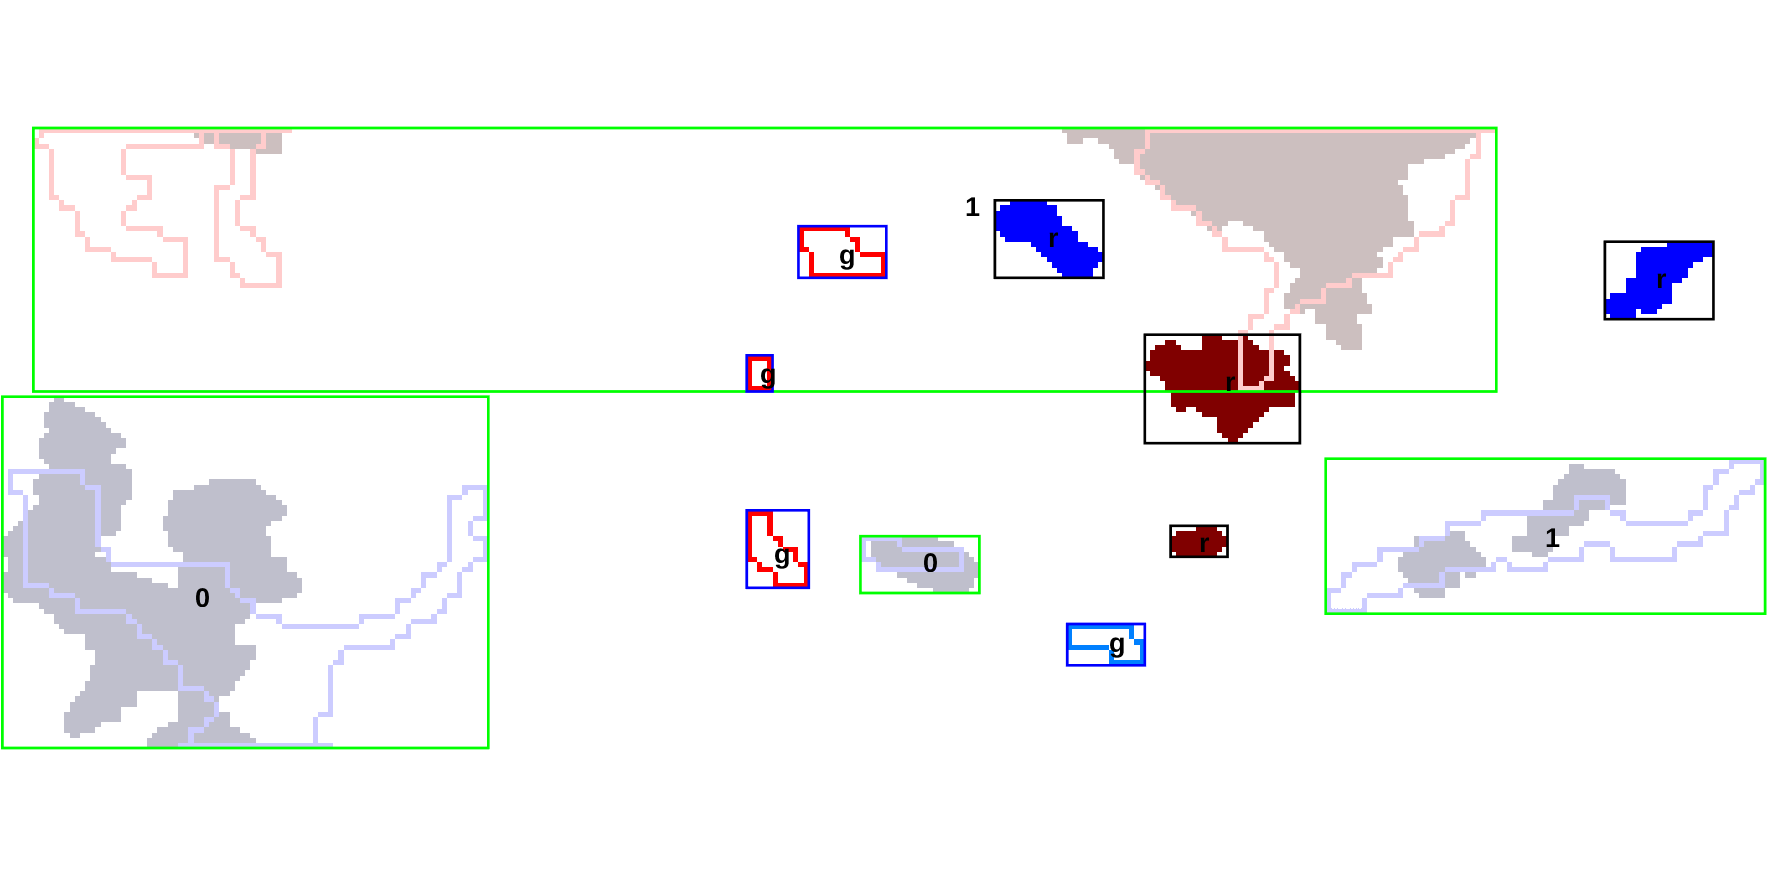
\includegraphics[width=0.45\linewidth]{pictures/thesis/chapter3/classificationProtocol/20110120model8Matched_cropped.png}
		\label{subfig:m8g1}
		
	}
	~\subfloat[Model 9 is in group A (rank=2, bad match).]
	{
		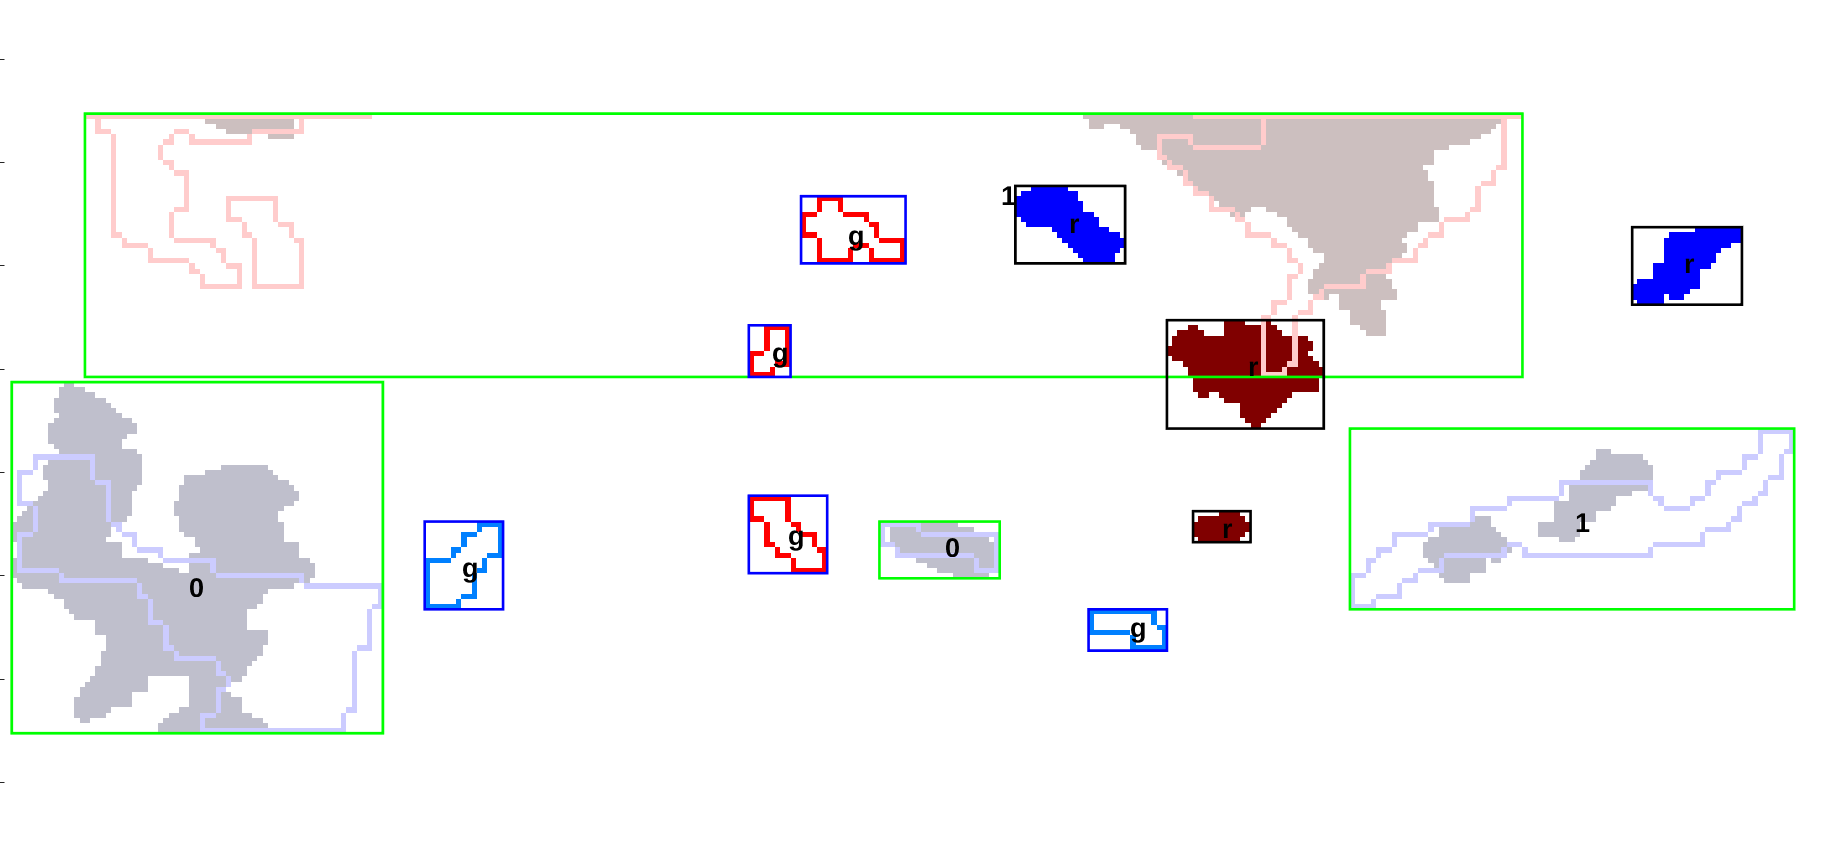
\includegraphics[width=0.45\linewidth]{pictures/thesis/chapter3/classificationProtocol/20110120model9Matched_cropped.png}
		\label{subfig:m9g1}
		
	}
	
	\subfloat[Model 11 is in group A (rank=2, bad match).]
	{
		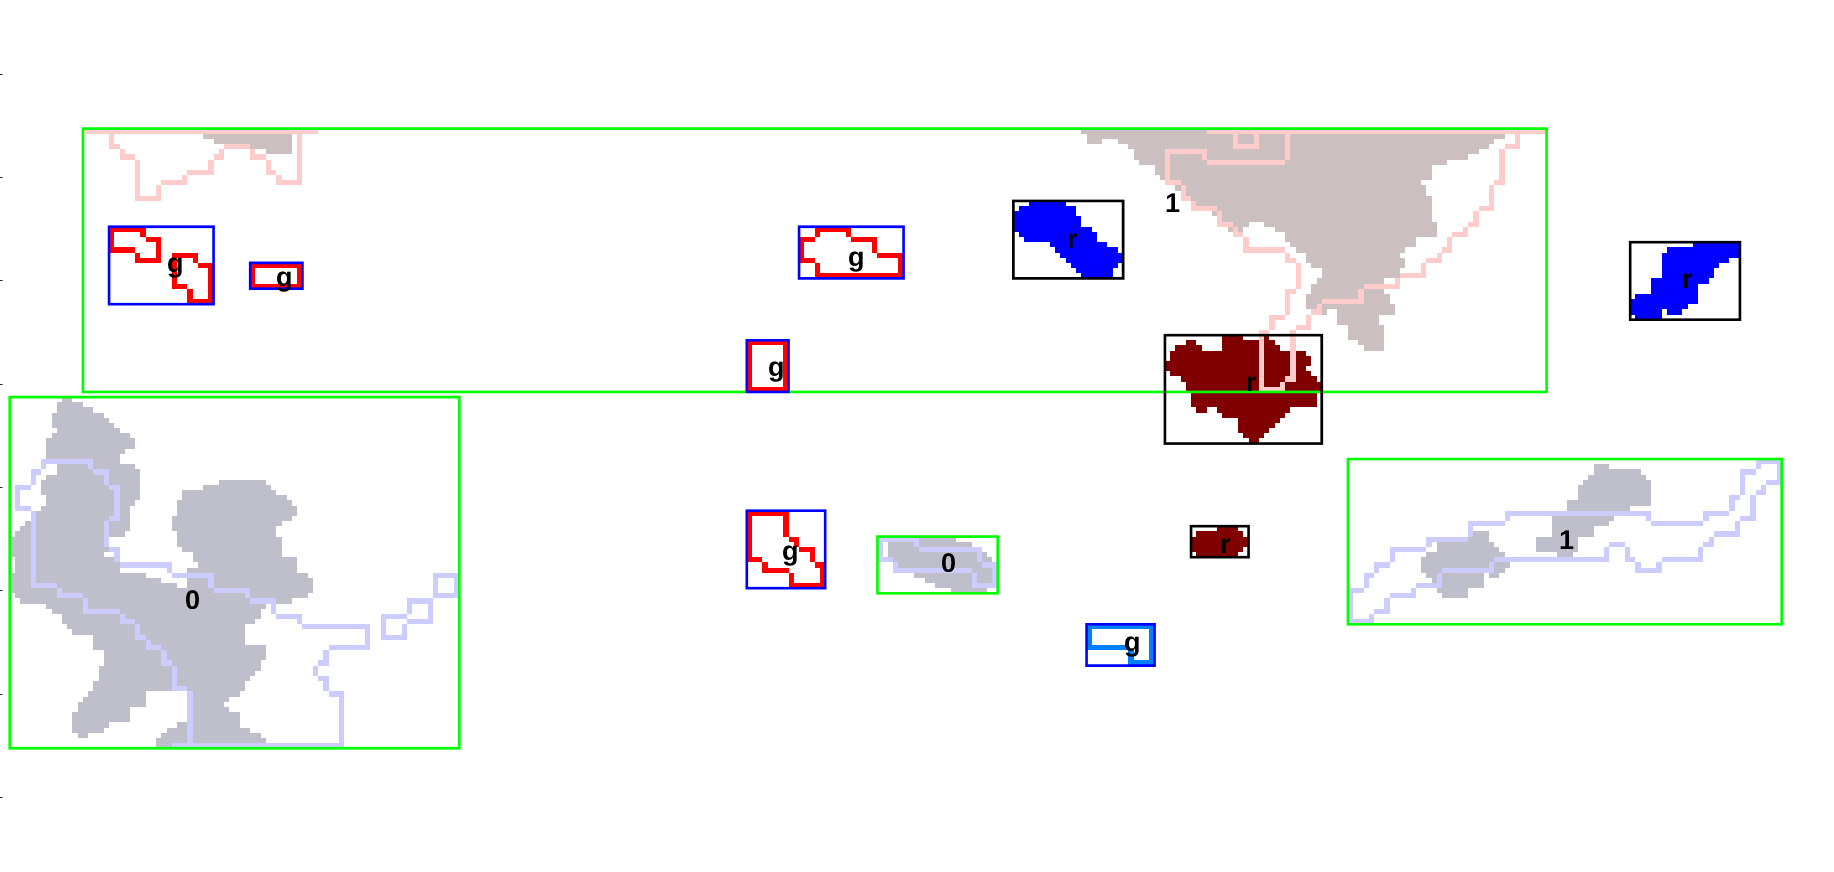
\includegraphics[width=0.45\linewidth]{pictures/thesis/chapter3/classificationProtocol/20110120model11Matched_cropped.png}
		\label{subfig:m11g1}
		
	}
	~\subfloat[Model 4 is in group B (rank=1, good match).]
	{
		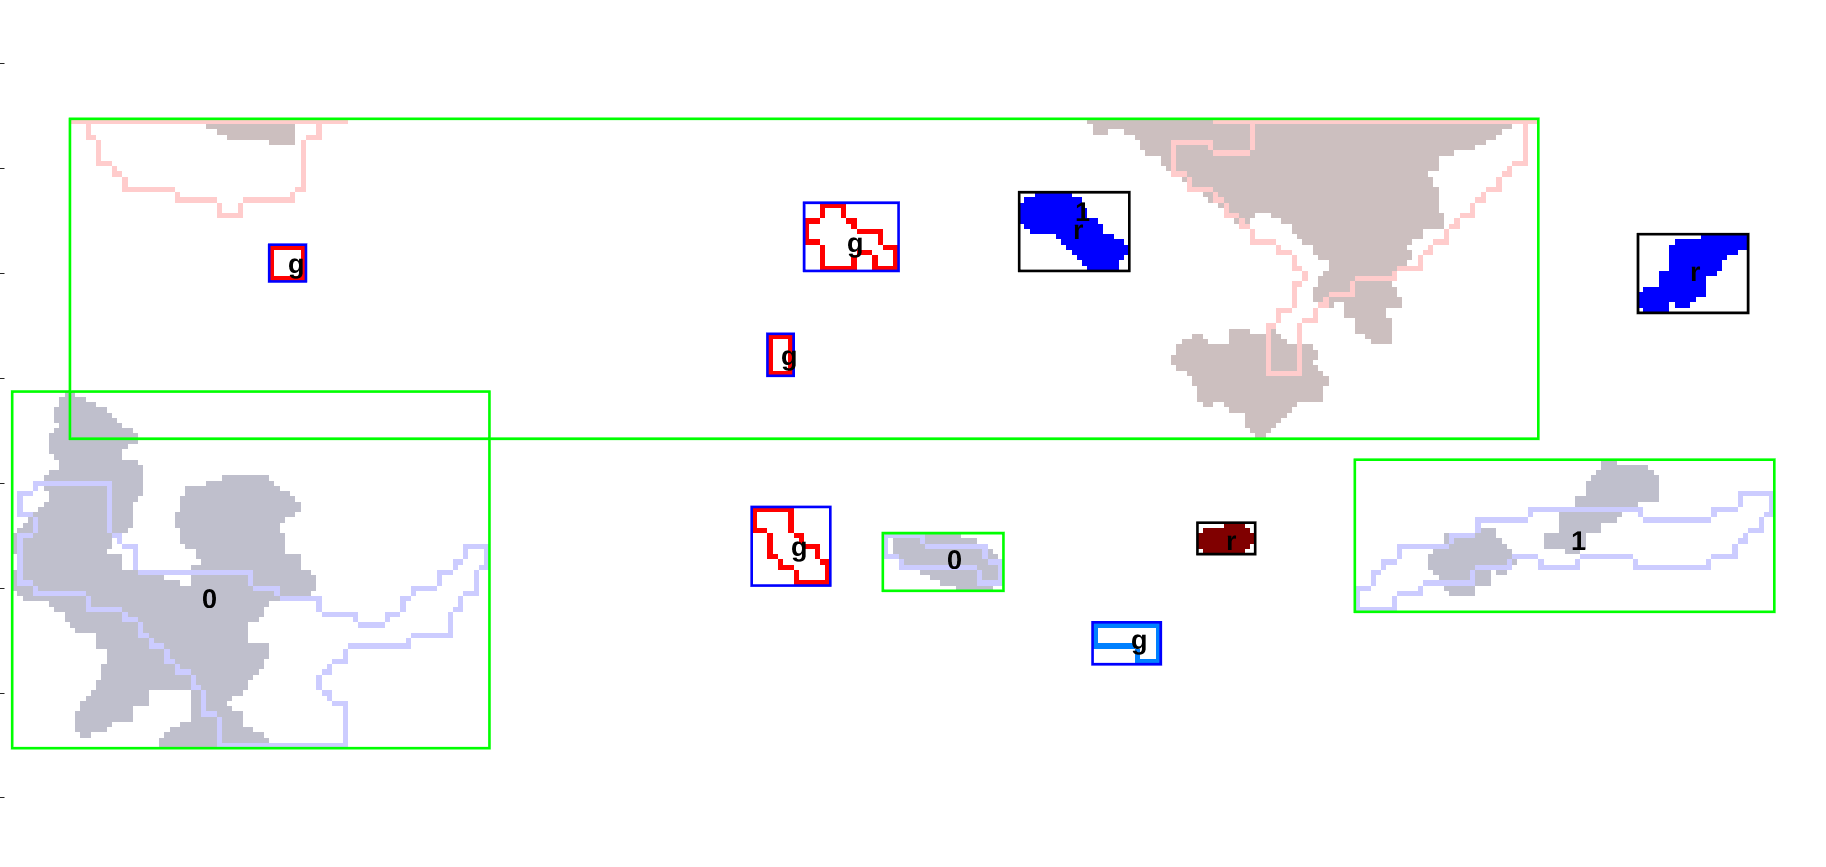
\includegraphics[width=0.45\linewidth]{pictures/thesis/chapter3/classificationProtocol/20110120model4Matched_cropped.png}
		\label{subfig:m4g2}
		
	}
	
	\subfloat[Model 10 is in group B (rank=1, good match).]
	{
		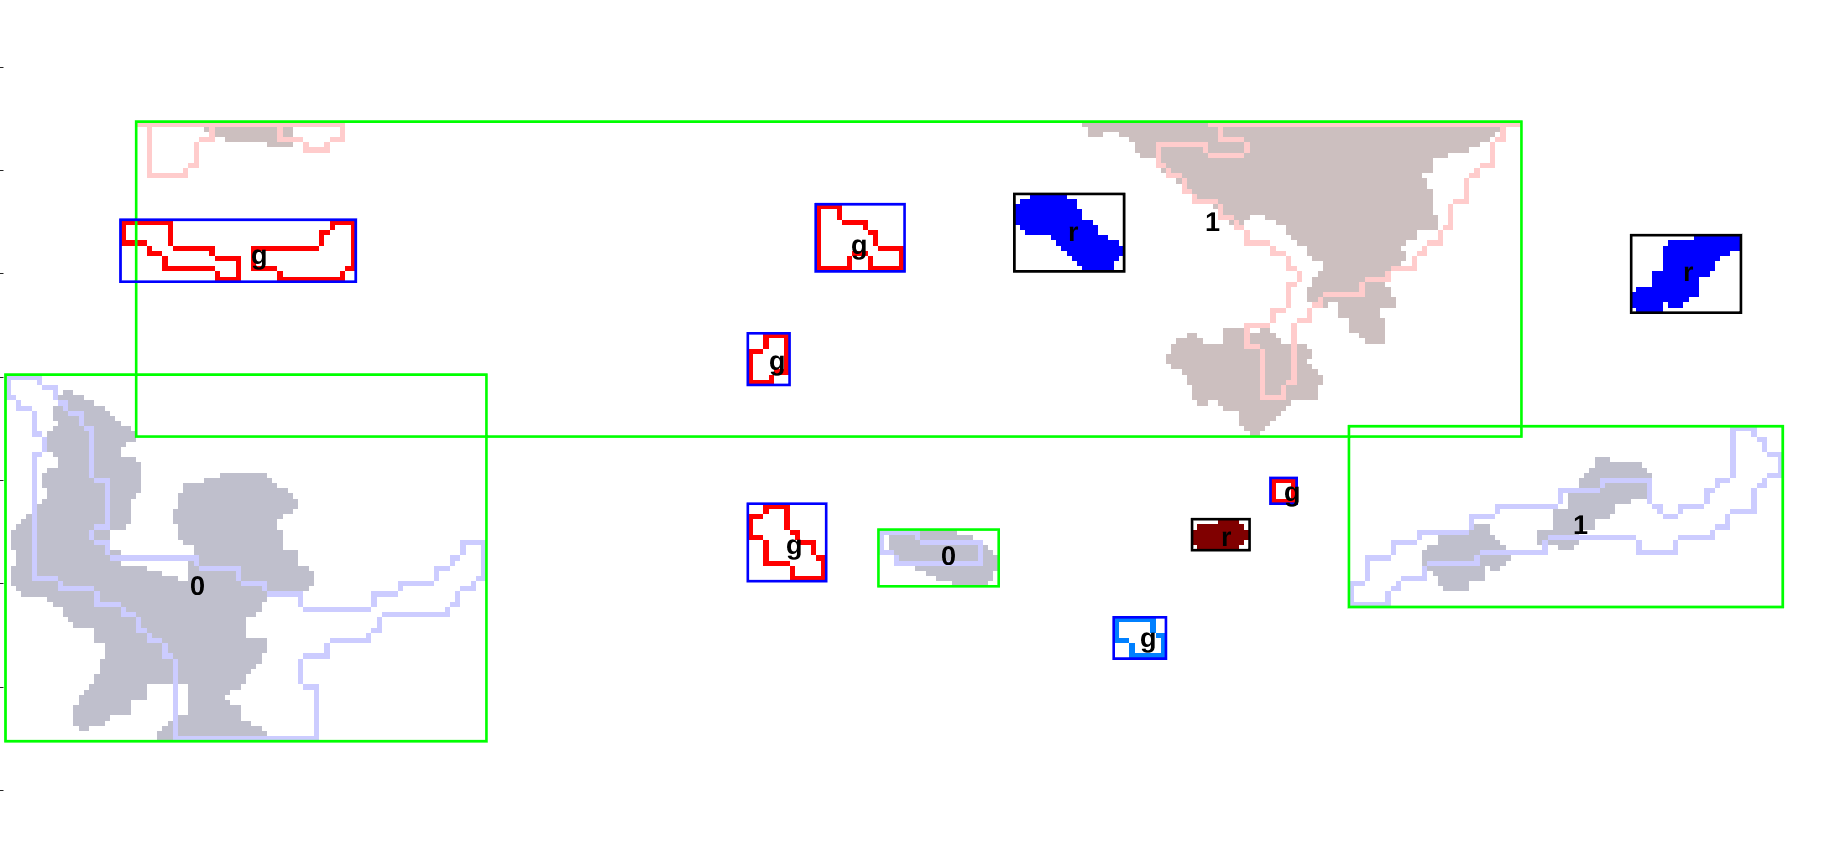
\includegraphics[width=0.45\linewidth]{pictures/thesis/chapter3/classificationProtocol/20110120model10Matched_cropped.png}
		\label{subfig:m10g2}
	}
	~\subfloat[Model 12 is in group B (rank=1, good match).]
	{
		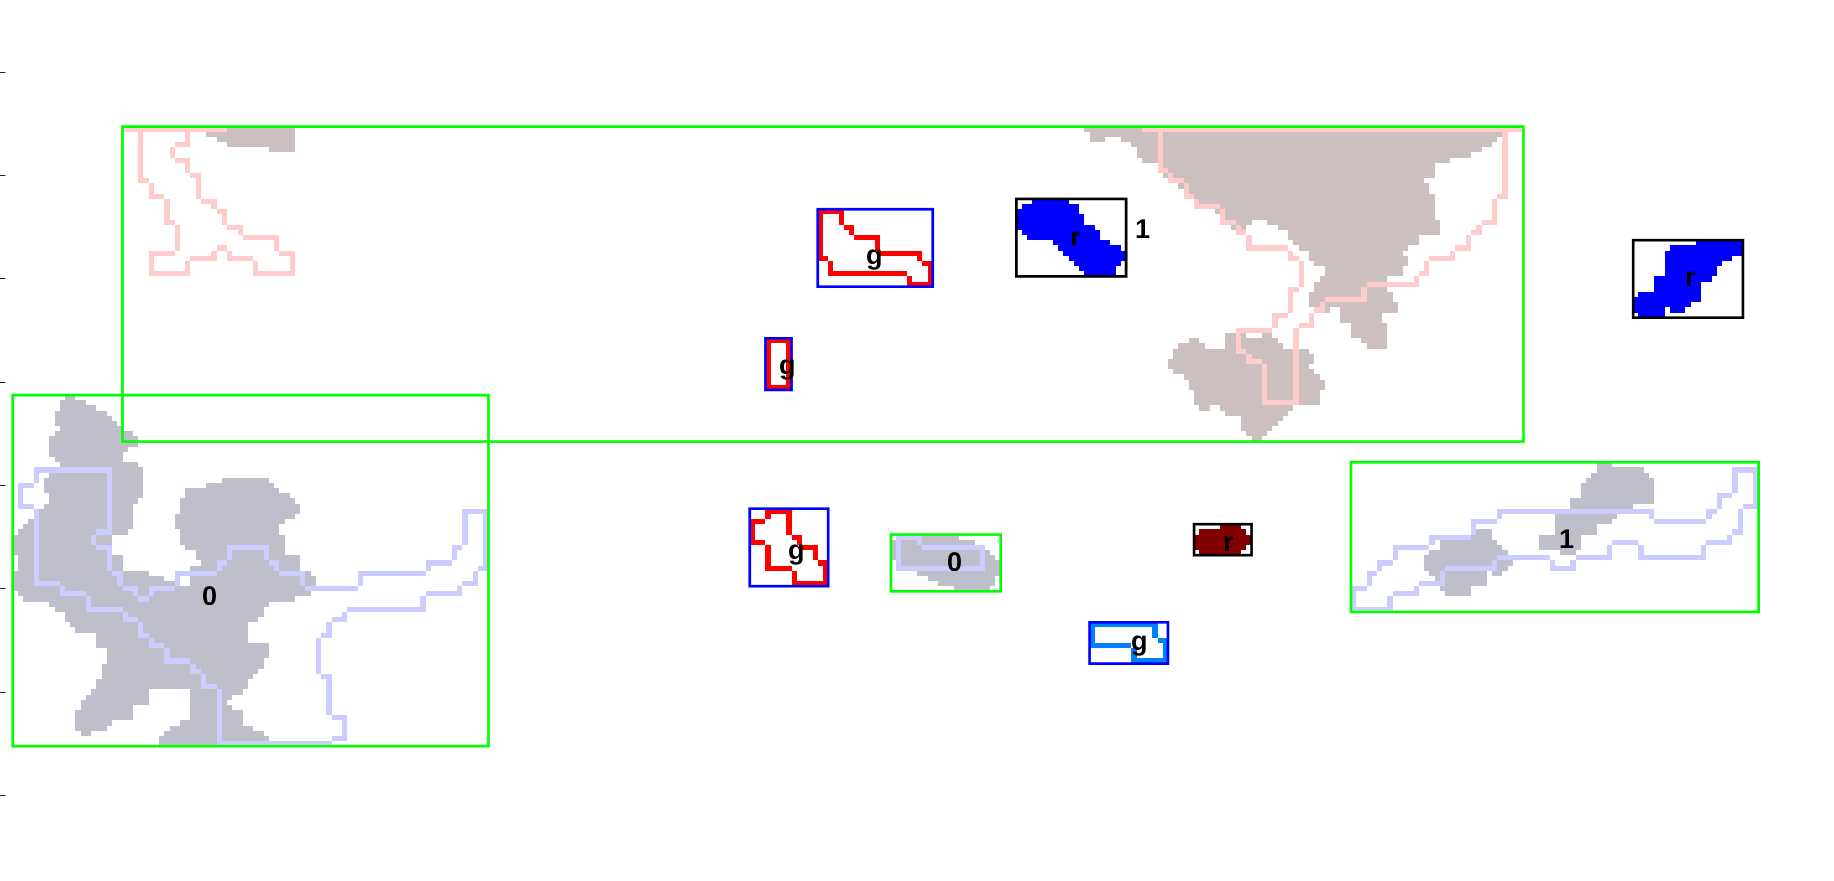
\includegraphics[width=0.45\linewidth]{pictures/thesis/chapter3/classificationProtocol/20110120model12Matched_cropped.png}
		\label{subfig:m12g2}
		
	}
	\caption{
	Map classification example (see Fig. \ref{fig:classAlg}).
	The maps are grouped into groups A and B.
	Group A is classified as rank 2.
	Group B is classified as rank 1. 
	Maps with rank 1 are classified as good.
	Maps with rank 2 are classified as bad. % date=1/20/2011. 
    }
	\label{fig:classificationInAction}
\end{figure}